\documentclass{article}
\usepackage{../../myPackage}


\begin{document}
%start of iteration 1
	\subsection{Emergency App - Video Streaming}
		\subsubsection{Iteration 1 - Basic Functionality}
			\paragraph{Aims}
			This iteration develops the core functionality of the video stream service. It is intended to provide the most basic features of making a video stream, with all the security operations implemented.\\

			At the most basic level, the user has to be able to start and stop the video stream and the operator has to be able to request the start and stop of the video stream and see it on his computer screen. Throughout this iteration, the following features are intended to be developed: the communication between the mobile devices and the server, encoding of the stream, basic UI for the backend and the mobile application and security measures such as creating emergency session for a given phone number and accepting only video streams from such phone number.
			
			\paragraph{Starting a video stream}
			Once a phone call with the emergency center has begun, the user has the option to start the application and choose to start streaming video. The operator will be able to see what the caller’s phone is capturing live on his screen. Apart from the user initiating the call, the operator will also be able to request the start of a video stream by sending a notification to the user’s phone.
	\begin{figure}[H]
		\centering
		\includegraphics[width=1\textwidth]{"EmergencyAppIteration1/iteration1backendsearch"}
	\end{figure}
	
Before a video stream can be initiated, the operator has to enter the caller’s phone number into the system. This will match the phone number with the user token into the database and will create a new session with a 2 minute time limit. The video stream has to be started during the time limit, or the session will expire and the user will not be able to start streaming. In such case, the operator has to initiate a new session for the user. This is done in order to check whether the user has the application installed on his phone and will minimize fake calls or misclicks by users.
	\begin{figure}[H]
		\centering
		\includegraphics[width=1\textwidth]{"EmergencyAppIteration1/sequenceinitiatesession (2)"}
		Sequence diagram 1. The operator creates a session.
	\end{figure}

There are two options in order to start the stream: Either the user opens the app and starts the stream manually, or the operator requests the sending of a notification to the user’s phone. After the user’s phone receives the notification, it will display a confirm dialog, which will start the video stream on confirmation.\\

In the second case, the server sends the notification through the Google Cloud Messaging (GCM) service. In order to do this, the server matches the phone number of the caller with its GCM \texttt{\color{OliveGreen}notification\_id} in the database and creates a message with a structure as shown below. The message is then sent and handled by the GCM service.
\begin{lstlisting}
...
"data":
      {
          "message_type":"video_call",
          "session_created_timestamp":"DATETIME",
          "session_time_limit":"TIME"
      }
...

\end{lstlisting}

\begin{wrapfigure}{l}{0.5\textwidth}
\vspace{-20pt}
  \begin{center}
    \includegraphics[width=0.48\textwidth]{"EmergencyAppIteration1/emergencydialog"}
  \end{center}
\vspace{-110pt}
\end{wrapfigure}
Once it is received by the mobile phone, the phone checks whether the notification is recent and correct by checking whether \texttt{\color{OliveGreen}session\_created\_timestamp} plus \texttt{\color{OliveGreen}session\_time\_limit} is past the current time. This will handle events, when the GCM service is unable to deliver the message instantly and the message arrives some time after the emergency call. In such case, the confirmation dialog won’t be displayed and the received notification will just be ignored.\\

When received on time, the notification will cause the opening of a confirmation dialog that will prompt the user to accept the video stream and if accepted it fires up the application automatically and starts streaming video, as if the user has started the application by himself. Apart from that, on accept or decline, the mobile phone will notify the server for its choice, in order to update the status of the operator’s request.

\pagebreak
\paragraph{Opening the Socket}
In order to initiate the video stream a Socket has to be opened, connecting the application with the server. Before the Socket can be opened, the user’s application needs the token, obtained when the user first installs the application and registers for the service. It is then encoded in the Secure Session Initiation Protocol’s URI Scheme as shown below. The server then checks whether the token matches any opened video stream session and will either accept it and start the stream, or will decline it.
\begin{lstlisting}
sips:<token>@<server_url>:<server_port>
\end{lstlisting}
If accepted, a Real-time Transport Protocol (RTP) [40] socket is opened between the client and the server. It is designed for handling audio and video communication over the network. To provide a reliable transfer of data, RTP provides error correction algorithms, used for lost packages, and integrated flow control, which ensures that packages are received in order. The above protocols provide Quality of Service (QoS) feedback, which can be used to adjust the quality of the video stream, based on the current internet connection. The protocols also provide Payload identification and Frame indication, which can be used to notify the receiver of any encoding, frame rate or frame size changes. The application will stream only video, as the audio call is already established over the phone and the application should not interrupt it.\\

Then the current settings for the stream and camera are sent over: frame size, frame rate and bitrate. Once the socket is opened and configured, the camera is started and streaming begins. The stream is encoded with VP9. We have chosen to use VP9 as a video compression technology over one of the most popular encoding techniques: H. 265, because VP9 is said to be more reliable for streaming [41].  VP9 is open source and royalty free video encoding format being developed by Google [42]. Youtube uses it for 4K resolution content. Matt Frost [43], senior business product manager for the Chrome Web Media Team, addresses audience at Google I/O: “People watch more than 4 billion YouTube videos a day and the company streams more than 6 billion hours of video each month”. "With a codec as good as VP9, we can significantly increase the size of the Internet," Frost said. "We can significantly increase the speed of the Internet". Based on statistics, VP9 doubles the quality of its predecessor VP8. Google in its own performance comparison claims that VP9 achieves over 50\% lower size of the video for the same quality when compared to H.264 [44]. This however, comes with the price of the compressing algorithm requiring more processing power.\\

On the server side, when the socket is opened and the initial settings are received, the system starts processing the data. Each packet is then decompressed and rendered onto the system’s interface. \\

The user and the operator are able to stop the video stream at any time, using the on-screen navigation on the app or the system interface, without interrupting the call itself.\\

	\begin{figure}[H]
		\centering
		\includegraphics[width=1\textwidth]{"EmergencyAppIteration1/sequencestartvideouser"}
		Sequence diagram 2. The user starts a video stream.
	\end{figure}


	\begin{figure}[H]
		\centering
		\includegraphics[width=1\textwidth]{"EmergencyAppIteration1/sequenceoperatorrequestvideo"}
		Sequence diagram 3. The operator requests the start of a video call.
	\end{figure}
	
	
	\begin{figure}[H]
		\centering
		\includegraphics[width=1\textwidth]{"EmergencyAppIteration1/sequenceoperatorrequestvideo"}
		Sequence diagram 3. The operator requests the start of a video call.
	\end{figure}

\begin{figure}
        \centering
        \begin{subfigure}[b]{0.5\textwidth}
                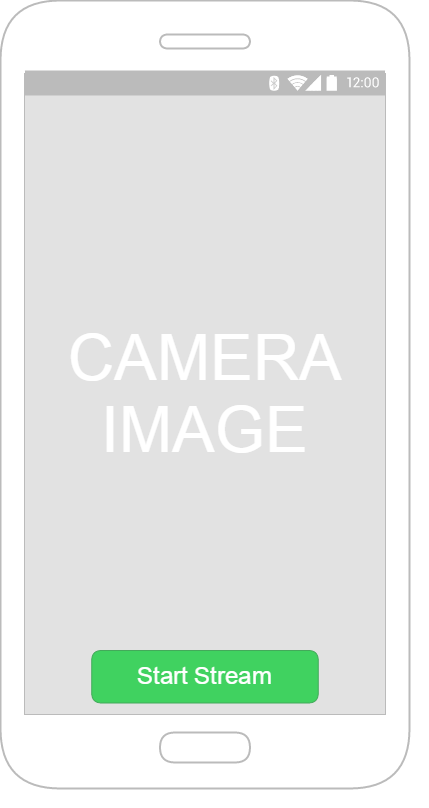
\includegraphics[width=\textwidth]{EmergencyAppIteration1/iteration1videocallStart}
        \end{subfigure}%
        ~ %add desired spacing between images, e. g. ~, \quad, \qquad, \hfill etc.
          %(or a blank line to force the subfigure onto a new line)
        \begin{subfigure}[b]{0.5\textwidth}
                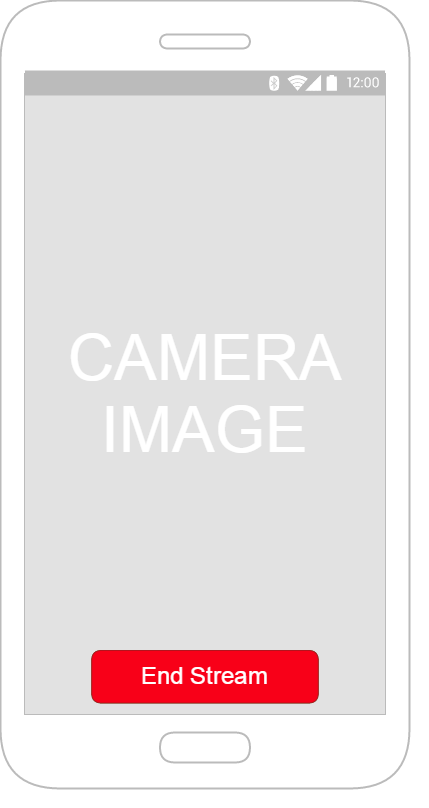
\includegraphics[width=\textwidth]{EmergencyAppIteration1/iteration1videocallEnd}
        \end{subfigure}
        Screens to manage the start and stop of the video stream by the user
\end{figure}


	\begin{figure}[H]
		\centering
		\includegraphics[width=.9\textwidth]{"EmergencyAppIteration1/iteration1backend"}
		
		Backend screen to request a video stream
	\end{figure}

	\begin{figure}[H]
		\centering
		\includegraphics[width=.9\textwidth]{"EmergencyAppIteration1/iteration1backend (1)"}
		
		Backend screen to stop the stream
	\end{figure}

	%iteration 2 start
	\pagebreak
	\subsubsection{Iteration 2 - Enhanced User Experience}
			\paragraph{Aims}
			This iteration aims at enhancing  the user experience during a video conversation. It includes setting up video stream quality and introducing video stream interface buttons.

			\paragraph{Setting the quality of the video stream}
			The user is able to change the prefered stream quality both in the application settings, when not in a call, and through the live stream interface, during a call. If the settings are not set manually, the quality is set automatically based on the mobile phone’s capabilities and the internet connection available.\\

The user will be able to choose between the following stream qualities: low, medium and high. Each of those will be set with unique frame rate, bitrate and resolution in order to optimize the performance and quality of the stream. A typical example of the importance of this feature is when a user is having a video stream and his internet connection is not very good, it would be reasonable that he changes the quality to medium or low, in order to keep the connection stable. This will also allow the user to minimize the used bandwidth, by choosing a lower quality setting.\\

High quality will mean encoding the video with a resolution of 720p (1280x720) [45] [39]. The video bit rates will be a maximum of 4000 kbps to a minimum of 1000 kbps, where the default will be 2500 kbps. The frames per second will be adjusted based on the device’s camera capabilities, but never exceeding 30 fps [46]. Medium quality option will provide a resolution of 360p (640x360) [45]. The video bit rates will be a maximum of 2000 kbps to a minimum of 500 kbps, where the default will be 1000 kbps. Low quality option will provide a resolution of 240p (320x180) [45]. The video bit rates will be a maximum of 1000 kbps to a minimum of 400 kbps, where the default will be 750 kbps. The video bitrates for the different quality options will be adjusted automatically by the application, based on the user’s internet connection.

\paragraph{Video Stream UI}
Apart from choosing the quality of the video stream, the user will be able to choose which camera of the phone to use, during the stream. The user interface during a video stream will allow the user to easily switch between cameras. Selecting a different camera will also affect the stream quality, as usually both cameras are not the same. If the user’s phone does not have a front camera, the button will not be available.\\

Another feature that the on-screen UI will provide, is switching the mobile phone’s flashlight on and off, in order for the user to be able to stream video in low light conditions. If the user’s phone does not have a flashlight, the flashlight button will not appear on his screen.
In order to make the call still available, while the user is streaming video and is holding his phone away from his ear, a button for enabling and disabling the loudspeaker has been included too.\\

All icons of the buttons included in the on-screen UI are the default icons used in many already existing applications that are using the camera. This way, they will be intuitive to the users and won’t need further description, which is an important point in the UI. If there are too many on-screen buttons, the picture won’t be clearly visible and the user may experience difficulties during the stream.\\

	\begin{figure}[H]
		\centering
		\includegraphics[width=.9\textwidth]{"EmergencyAppIteration2/iteration2ui (1)"}
		
		On screen UI during a stream
	\end{figure}

	\begin{figure}[H]
		\centering
		\includegraphics[width=.6\textwidth]{"EmergencyAppIteration2/iteration2uisettings"}
		
		Stream quality settings
	\end{figure}


	%iteration 3 start
	\pagebreak
	\subsubsection{Iteration 3 - Enhanced Dispatcher Experience}
			\paragraph{Aims}
			The aims of this iteration is to provide the functionality of skipping and seeking through a live video stream and being able to review old videos.

\paragraph{Video storage and skip/seek to a certain time}
			As some emergency scenes may need further attention, all video streams will need to be stored. \\

In order to do this, a storage server will be needed, that is separate from the one running the backend UI or the database server. It will also need to be extendible, in order to include more storage devices or replace old ones.\\

The video stream will be saved immediately after the server receives it from the client and will continue writing to the same file, until the stream has been stopped. This will ensure that all streams are always saved and that if the backend UI crashes, the stream will still be saved and accessible. Each saved video stream will be labeled by its date and time, as well as with the ID of the operator taking the call. An example stream started on 21/04/2015 at 13:11 by an operator with ID 123456789, would look like:
\begin{lstlisting}
2015-04-21-13-11-123456789.webm
\end{lstlisting}
The WebM file format is a container for VP9 video streams and will be used when storing the video streams [47] [48].\\

The name of the file will be saved in the corresponding incident in the database and it will be searchable in our system’s user interface. \\

Moreover, even during the live video stream, operators will be able to skip/seek through the already recorded video and return to live footage at any time they want. This could be very beneficial, when something needs to be examined in depth, while the video stream is still in progress. When the operator chooses to go to a certain time of the stream, while it is still active, the live video will continue to be shown in a box in the top right corner of the main video window, while the scene that is chosen starts in the main one. This way the operator can see what is being streamed live and return to it immediately if necessary.\\

Licensed system’s users will have access to old recorded streams for further investigation. Reviewing can be done either by playing the file directly from the storage device with a third party software, or by using the user interface to search for it and play it.\\
			

	\begin{figure}[H]
		\centering
		\includegraphics[width=.9\textwidth]{"EmergencyAppIteration3/backend_videocall_nochat (1)"}
		
		Seeking back to a past moment of the stream
	\end{figure}
	\begin{figure}[H]
		\centering
		\includegraphics[width=.9\textwidth]{"EmergencyAppIteration3/backend_find_video_footage (1)"}
		
		Accessing old emergency sessions
	\end{figure}
			
	%iteration 4 start
	\pagebreak
	\subsubsection{Iteration 4 - Improving Reliability}
			\paragraph{Aims}
			This iteration aims at improving the reliability of the backend and the mobile application.

		\paragraph{Restore on unexpected close}
		There are events when computers may fail and the backend can close unexpectedly, closing the current emergency window. Such events include power cut, software bug or any hardware failure. As other actions can be taken in order to minimise the possibility of such event happening, the software by itself has to be able to react to it too. To do this, the system will adopt some new features.\\

Apart from that, the mobile application may face similar issues and restoring to the current emergency session, when the application has been closed or has crashed is an important feature.\\

Each operator will be able to open only one emergency session at a time. He will not be able to open or start another session, until he has closed the current one. In order to provide this functionality, the operator will need to explicitly state that he wants to close the emergency session. This will be done by a Dialog, which pops up when the back button has been clicked during the stream. The dialog will provide 3 options: Close the current emergency session, Go back and leave the current session opened, Stay on the page and close the dialog.\\

In the main screen, the operator will be able to see if there is a current active session and will be able to open it. This will help reopen the session in the case of a crash of the program or when the operator closed the windows, leaving the session open. The user can continue streaming during this time, as the server will continue processing the data. After opening the session again, the operator will be able to skip/seek back and see what has happened during the time his stream window was closed.\\

If the mobile application of the user crashes, on restart it will automatically try to reopen the stream.\\
	\begin{figure}[H]
		\centering
		\includegraphics[width=.9\textwidth]{"EmergencyAppIteration4/iteration4backendconfirmdialog (1)"}
		
		Confirmation of closing the session or navigating back
	\end{figure}
	\begin{figure}[H]
		\centering
		\includegraphics[width=.9\textwidth]{"EmergencyAppIteration4/current_session_search_screen"}
		
		 Notification of a current session
	\end{figure}
	
	
	
	%iteration 4 start
	\pagebreak
	\subsubsection{Iteration 5 - Multiple Live Streams}
			\paragraph{Aims}
			Give the operator the opportunity to switch between multiple live streams, that are showing the same emergency. This will allow for the operator to assess the severity of the incident even better and he will be able to react properly.
			
			\paragraph{Multiple Streams}
			When multiple operators take calls, there might be the case when two calls are actually about the same incident. As there is a way of marking two calls as the same incident in the current systems, we decided to implement a way of combining the information from different streams.\\

When an operator has opened a stream, he will be able to see whether there are other streams for the same incident and will be able to click them and review them. He will be able to watch the live stream, as well as skip/seek to a certain part of the stream. This is possible as all the streams are being saved on the storage server and if two streams are being marked as one incident, they will become accessible by the operators handling the calls.\\

The backend user interface will allow to chose different streams and watch them, while the current live stream will remain as a thumbnail and the operator will be able to return to it with only one click. Every alternative stream will be marked by the unique telephone number that the user is calling from.\\

	\begin{figure}[H]
		\centering
		\includegraphics[width=.9\textwidth]{"EmergencyAppIteration5/more_accident_streams_iteration3 (1)"}
		
		Confirmation of closing the session or navigating back
	\end{figure}
	\begin{figure}[H]
		\centering
		\includegraphics[width=.9\textwidth]{"EmergencyAppIteration5/more_accident_streams_opened_iteration3"}
		
		 Notification of a current session
	\end{figure}




	\subsection{Emergency App - Chat}
		\subsubsection{Iteration 1 - Basic Functionality}
			\paragraph{Aims}
			This iteration develops the core functionality of starting a live chat with an emergency operator. It is intended to provide the user with alternative ways of holding a conversation, when he is in an emergency situation.

At the most basic level, a user should be able to begin an online chat conversation with an emergency operator. Moreover, the operator should be instantly notified when a chat session has begun. 

		\paragraph{Starting a live chat with an emergency operator}
		Once a user’s device has been registered, a chat conversation with an emergency team can be started. A user has to simply start the application and choose the emergency chat option. This will transfer him to a chat window, where he can start typing and send messages to 999. 

In order to establish the connection between the server and the application, a WebSocket [54] will be opened between them. Through it, messages can be sent over in real time. It is designed on top of TCP, which provides reliability for delivering the messages and ensures that they arrive in the correct order. This is very important for the emergency chat, as notifying the user if a message has been delivered, can greatly increase reaction time. The WebSocket will be opened through the following URI:
\begin{lstlisting}
	wss://<server-address>:<port>
\end{lstlisting}
This opens an encrypted connection between the client and the server. Once a connection has been established, the user has to identify himself. To do this, the application sends the id received when registering during the first start of the application. The server will respond with the ID of the emergency session created for the current emergency chat. All messages will be sent in the JSON format and will contain authorization token.\\

Request from the application to start an emergency chat:
\begin{lstlisting}
	{
          "Type":"start_session"
	}
\end{lstlisting}

Response from the server:
\begin{lstlisting}
	{
          "IncidentID":"abcd1234567890", -- Can be null if initiating a session was unsuccessful
          "Type":"session",
          "Status":"open/failed"
	}
\end{lstlisting}
After the session has been initiated, the user can start typing the emergency messages. Once the user starts typing a message, a notification is being sent, that the current Emergency chat is active and requiring operator’s attention. This is done in order to shorten the response time, by notifying the call center of new emergency chats, before the actual message has been received.\\

Application notifies the server for an active chat:
\begin{lstlisting}
      {
          "IncidentID":"abcd1234567890",
          "Type":"session",
          "Status":"active"
      }
\end{lstlisting}

The information can then be sent in multiple messages, sending each bit of information as a separate message. The example given on the Emergency SMS website [51] can be broken down into the following messages:\\

Original: 'ambulance. man having a heart attack. outside post office. valley road watford'\\

Chat messages:
\begin{enumerate}

\item ambulance
\item man having heart attack
\item valley road watford
\item outside post office

\end{enumerate}
This will allow for the operator to respond faster. When the message requesting an ambulance has been received, the operator can react accordingly and record the emergency in the system. When the description and the location has been received, the operator can quickly contact the emergency team in the corresponding region or ask for more information in just a few seconds. A simple chat message will also provide delivery report, as well as an indicator if the operator has opened the chat or not, which will allow the user to get faster information on whether the messages were delivered. If the message fails to be delivered, the application will retry to send it automatically, without the need of the user typing the message again. However, if the message fails to be accepted by the server for any other reason, a notification will appear on the user’s screen, describing the error.\\

Simple outgoing chat message (both from operator or from user):
\begin{lstlisting}
	{
          "IncidentID":"session1234567890",
          "Type":"message",
          "Message":"need ambulance",
          "Timestamp":"437647234",
          "TempMessageID":"temp1234567890"
	}
\end{lstlisting}

Delivery confirmation message (sent to the sender of the message):
\begin{lstlisting}
	{
          "IncidentID":"session1234567890",
          "Type":"message_report",
          "TempMessageID":"temp1234567890",
          "MessageID":"message1234567890",
          "Status":"delivered/failed",
          "Error":"A description, which will be displayed in a popup." -- If message was delivered, this field is empty
	}
\end{lstlisting}

Operator connected message (sent to user, once an operator opens the emergency chat session:
\begin{lstlisting}
	{
          "IncidentID":"session1234567890",
          "Type":"message_report",
          "MessageID":"message1234567890",
          "Status":"seen"
	}
\end{lstlisting}
The user will be able to close the application at any one moment, however, the emergency session will be active until the operator decides to close it. If the user closes the application and tries to start a new chat session, while his current session is active, he will send the messages to the same operator and the same emergency session. This will handle accidental closes or crashes of the applications and will allow the user to go back to the conversation.

\paragraph{Sending a notification for a started chat session}
On the operator side, when the user selects chat option and starts typing, there is a notification that pops up that informs the operator that there is an emergency going on and that there are incoming messages. These notifications are acquired by getting all incident sessions with a status of pending chat.

	\begin{figure}[H]
		\centering
		\includegraphics[width=1\textwidth]{"ChatIteration1/chat_backend_search"}
		
		Backend notifies of new pending chats
	\end{figure}
When the operator selects to respond a chat, he is assigned an emergency session. In order to avoid multiple operators responding to one chat, transactions are used. When the operator responds to a chat, there is a transaction that is being sent to the database, that locks the session only for that operator. Transactions are the way to ensure that the users of the system are working with consistent information and provide error recovery mechanisms. The distribution works the following way: 
\begin{enumerate}
\item The user sends a message.
\item The message travels to the emergency center.
\item The systems identifies available operators and notifies them that they can start an emergency chat.
\item The operator selects to start a chat.
\item A chat session starts and becomes private only to that operator, while it is being handled.
\item When the emergency has been handled and the operator closes the session, the user will not be able to send any more messages in the current session.

\end{enumerate}
The backend will allow the operator to simultaneously use both the video stream service and the chat service, which will ensure that no time is wasted for switching between screens.

	\begin{figure}[H]
		\centering
		\includegraphics[width=1\textwidth]{"ChatIteration1/backend_video_call (1)"}
		
		Both video streaming and live chat will be available to the operator in the same window
	\end{figure}

\end{document}
